%% Valve containment in liquid diaphragm pumps: contact on a signed distance field, on Grace and
%% Hopper.
%%
%% Build:  make          (latexmk -pdf)
%%         make figures  (regenerate every figure, table and macro from data/)
%%
%% NOTHING IN THIS FILE IS A TYPED-IN MEASUREMENT. Every measured quantity arrives through
%% \input{tables/...} or a macro of figures/ldp_macros.tex, emitted by python/ldp_figures.py from
%% data/, so a re-measurement propagates. README.md names the job behind each data file.
\documentclass[sigconf,nonacm]{acmart}

\usepackage{tikz}
\usepackage{pgfplots}
\pgfplotsset{compat=1.18}
\usepackage{booktabs}
\usepackage{siunitx}
\sisetup{group-separator={,},group-minimum-digits=4,group-digits=integer}
\usepackage{draftwatermark}
\SetWatermarkText{DRAFT}
\SetWatermarkScale{1.1}
\SetWatermarkLightness{0.93}

%% Generated by wip/ldp_containment/python/ldp_figures.py -- do not edit.
%% Regenerate with: make figures
\definecolor{LdpA}{HTML}{4C72B0}
\definecolor{LdpB}{HTML}{DD8452}
\definecolor{LdpC}{HTML}{55A868}
\definecolor{LdpD}{HTML}{C44E52}

%% Generated by wip/ldp_containment/python/ldp_figures.py -- do not edit.
%% Regenerate with: make figures
\newcommand{\machineCPU}{Neoverse-V2}
\newcommand{\machineModules}{4}
\newcommand{\machineCores}{72}
\newcommand{\machineHostMemory}{\SI{856}{\giga\byte}}
\newcommand{\machineGPU}{GH200 120GB}
\newcommand{\machineGPUMemory}{\SI{96}{\gibi\byte}}
\newcommand{\machineDriver}{595.91.07}
\newcommand{\machineCUDA}{12.6}
\newcommand{\machineGCC}{13.3.0}
\newcommand{\machineMPICH}{8.1.30}
\newcommand{\machineLibfabric}{1.15.2.0}
\newcommand{\benchRepeats}{3}
\newcommand{\benchRuns}{\num{120}}
\newcommand{\benchFailed}{\num{0}}
\newcommand{\benchSpread}{\num{7.6}}
\newcommand{\benchSpreadMedian}{\num{1.8}}
\newcommand{\benchSpreadWhere}{FP70, $4\times72$}
\newcommand{\elementsFFc}{\num{242336}}
\newcommand{\dofsFFc}{\num{150525}}
\newcommand{\contactFFc}{\num{18780}}
\newcommand{\newtonFFc}{\num{20}}
\newcommand{\qpFFc}{\num{11549}}
\newcommand{\qpSpreadFFc}{\num{16}}
\newcommand{\elementsFPc}{\num{384001}}
\newcommand{\dofsFPc}{\num{223332}}
\newcommand{\contactFPc}{\num{20163}}
\newcommand{\newtonFPc}{\num{10}}
\newcommand{\qpFPc}{\num{15603}}
\newcommand{\qpSpreadFPc}{\num{7.2}}
\newcommand{\elementsFPf}{\num{948944}}
\newcommand{\dofsFPf}{\num{526809}}
\newcommand{\contactFPf}{\num{33479}}
\newcommand{\newtonFPf}{\num{4}}
\newcommand{\qpFPf}{\num{4344}}
\newcommand{\qpSpreadFPf}{\num{21}}
\newcommand{\elementsFFf}{\num{1768274}}
\newcommand{\dofsFFf}{\num{973812}}
\newcommand{\contactFFf}{\num{57066}}
\newcommand{\newtonFFf}{\num{16}}
\newcommand{\qpFFf}{\num{28166}}
\newcommand{\qpSpreadFFf}{\num{17}}
\newcommand{\qpSpreadMax}{\num{21}}
\newcommand{\dofsMin}{\num{150525}}
\newcommand{\dofsMax}{\num{973812}}
\newcommand{\dofsRatio}{\num{6.5}}
\newcommand{\convergedCases}{FF200, FP70 coarse and FF200 refined}
\newcommand{\unconvergedCases}{FP70}
\newcommand{\convergedTol}{\num{1e-6}}
\newcommand{\qpCap}{\num{15000}}
\newcommand{\qpCapped}{\num{0}}
\newcommand{\qpCappedClause}{no QP solve reaches the iteration cap of \num{15000}}
\newcommand{\agreeSerial}{\num{1.6e-7}}
\newcommand{\agreeParallel}{\num{7.6e-7}}
\newcommand{\agreeParallelAbs}{\num{3.1e-10}}
\newcommand{\agreeUnconverged}{\num{0.0050}}
\newcommand{\finalUnconverged}{\num{0.0023}}
\newcommand{\coordUlp}{\num{1.2e-10}}
\newcommand{\coordUlpMax}{\num{1.9e-9}}
\newcommand{\abRelMaxFPc}{\num{8.3}}
\newcommand{\abRelLFPc}{\num{3.8}}
\newcommand{\abRelMaxFPf}{\num{7.4}}
\newcommand{\abRelLFPf}{\num{4.2}}
\newcommand{\abRelMaxFFc}{\num{3.9}}
\newcommand{\abRelLFFc}{\num{2.3}}
\newcommand{\abRelMaxFFf}{\num{4.2}}
\newcommand{\abRelLFFf}{\num{0.83}}
\newcommand{\abPenUtopiaMax}{\num{6.1e-6}}
\newcommand{\abSdfSfemMax}{\num{-2.6e-6}}
\newcommand{\abJaccardMin}{\num{0.957}}
\newcommand{\kktUtopiaFPc}{\num{0.030}}
\newcommand{\kktSfemFPc}{\num{4.9e-7}}
\newcommand{\kktUtopiaFPf}{\num{0.024}}
\newcommand{\kktSfemFPf}{\num{0.0069}}
\newcommand{\kktUtopiaFFc}{\num{0.092}}
\newcommand{\kktSfemFFc}{\num{9.3e-9}}
\newcommand{\kktUtopiaFFf}{\num{0.099}}
\newcommand{\kktSfemFFf}{\num{6.6e-9}}
\newcommand{\kktRatioMin}{\num{61000}}
\newcommand{\kktRatioMax}{\num{1.5e7}}
\newcommand{\kktGridChange}{\num{0.07}}
\newcommand{\utopiaTimeFPc}{\num{128}}
\newcommand{\utopiaNewtonFPc}{\num{10}}
\newcommand{\utopiaTimeFPf}{\num{243}}
\newcommand{\utopiaNewtonFPf}{\num{4}}
\newcommand{\utopiaTimeFFc}{\num{80.9}}
\newcommand{\utopiaNewtonFFc}{\num{4}}
\newcommand{\utopiaTimeFFf}{\num{680}}
\newcommand{\utopiaNewtonFFf}{\num{4}}
\newcommand{\utopiaRanks}{\num{8}}
\newcommand{\itFFcHostOne}{\num{171}}
\newcommand{\tFFcHostOne}{\num{2.69}}
\newcommand{\itFFcHostFour}{\num{242}}
\newcommand{\tFFcHostFour}{\num{3.27}}
\newcommand{\itFFcHostSixteen}{\num{137}}
\newcommand{\tFFcHostSixteen}{\num{2.09}}
\newcommand{\itFFcHostFourTwo}{\num{222}}
\newcommand{\tFFcHostFourTwo}{\num{3.18}}
\newcommand{\itFFcHostEight}{\num{292}}
\newcommand{\tFFcHostEight}{\num{4.04}}
\newcommand{\itFFcHostThirtyTwo}{\num{199}}
\newcommand{\tFFcHostThirtyTwo}{\num{2.87}}
\newcommand{\itFFcGpuOne}{\num{85}}
\newcommand{\tFFcGpuOne}{\num{1.38}}
\newcommand{\itFFcGpuFour}{\num{139}}
\newcommand{\tFFcGpuFour}{\num{2.42}}
\newcommand{\itFFcGpuFourTwo}{\num{131}}
\newcommand{\tFFcGpuFourTwo}{\num{2.08}}
\newcommand{\itFFcGpuEight}{\num{159}}
\newcommand{\tFFcGpuEight}{\num{2.91}}
\newcommand{\bestFFc}{1 GPU}
\newcommand{\bestTimeFFc}{\num{1.38}}
\newcommand{\gpuOverGraceFFc}{\num{1.5}}
\newcommand{\qpShareFFc}{\num{68}}
\newcommand{\itFPcHostOne}{\num{212}}
\newcommand{\tFPcHostOne}{\num{3.75}}
\newcommand{\itFPcHostFour}{\num{243}}
\newcommand{\tFPcHostFour}{\num{4.16}}
\newcommand{\itFPcHostSixteen}{\num{162}}
\newcommand{\tFPcHostSixteen}{\num{2.87}}
\newcommand{\itFPcHostFourTwo}{\num{230}}
\newcommand{\tFPcHostFourTwo}{\num{3.87}}
\newcommand{\itFPcHostEight}{\num{276}}
\newcommand{\tFPcHostEight}{\num{4.69}}
\newcommand{\itFPcHostThirtyTwo}{\num{192}}
\newcommand{\tFPcHostThirtyTwo}{\num{3.34}}
\newcommand{\itFPcGpuOne}{\num{99}}
\newcommand{\tFPcGpuOne}{\num{1.81}}
\newcommand{\itFPcGpuFour}{\num{141}}
\newcommand{\tFPcGpuFour}{\num{3.10}}
\newcommand{\itFPcGpuFourTwo}{\num{132}}
\newcommand{\tFPcGpuFourTwo}{\num{2.50}}
\newcommand{\itFPcGpuEight}{\num{172}}
\newcommand{\tFPcGpuEight}{\num{3.51}}
\newcommand{\bestFPc}{1 GPU}
\newcommand{\bestTimeFPc}{\num{1.81}}
\newcommand{\gpuOverGraceFPc}{\num{1.6}}
\newcommand{\qpShareFPc}{\num{72}}
\newcommand{\itFPfHostOne}{\num{531}}
\newcommand{\tFPfHostOne}{\num{2.77}}
\newcommand{\itFPfHostFour}{\num{299}}
\newcommand{\tFPfHostFour}{\num{1.75}}
\newcommand{\itFPfHostSixteen}{\num{211}}
\newcommand{\tFPfHostSixteen}{\num{1.31}}
\newcommand{\itFPfHostFourTwo}{\num{278}}
\newcommand{\tFPfHostFourTwo}{\num{1.63}}
\newcommand{\itFPfHostEight}{\num{322}}
\newcommand{\tFPfHostEight}{\num{1.94}}
\newcommand{\itFPfHostThirtyTwo}{\num{220}}
\newcommand{\tFPfHostThirtyTwo}{\num{1.38}}
\newcommand{\itFPfGpuOne}{\num{173}}
\newcommand{\tFPfGpuOne}{\num{1.08}}
\newcommand{\itFPfGpuFour}{\num{181}}
\newcommand{\tFPfGpuFour}{\num{1.68}}
\newcommand{\itFPfGpuFourTwo}{\num{163}}
\newcommand{\tFPfGpuFourTwo}{\num{1.17}}
\newcommand{\itFPfGpuEight}{\num{174}}
\newcommand{\tFPfGpuEight}{\num{1.67}}
\newcommand{\bestFPf}{1 GPU}
\newcommand{\bestTimeFPf}{\num{1.08}}
\newcommand{\gpuOverGraceFPf}{\num{1.2}}
\newcommand{\qpShareFPf}{\num{50}}
\newcommand{\itFFfHostOne}{\num{1254}}
\newcommand{\tFFfHostOne}{\num{35.6}}
\newcommand{\itFFfHostFour}{\num{423}}
\newcommand{\tFFfHostFour}{\num{12.2}}
\newcommand{\itFFfHostSixteen}{\num{320}}
\newcommand{\tFFfHostSixteen}{\num{9.89}}
\newcommand{\itFFfHostFourTwo}{\num{405}}
\newcommand{\tFFfHostFourTwo}{\num{11.9}}
\newcommand{\itFFfHostEight}{\num{418}}
\newcommand{\tFFfHostEight}{\num{12.3}}
\newcommand{\itFFfHostThirtyTwo}{\num{297}}
\newcommand{\tFFfHostThirtyTwo}{\num{9.57}}
\newcommand{\itFFfGpuOne}{\num{278}}
\newcommand{\tFFfGpuOne}{\num{8.24}}
\newcommand{\itFFfGpuFour}{\num{203}}
\newcommand{\tFFfGpuFour}{\num{6.56}}
\newcommand{\itFFfGpuFourTwo}{\num{196}}
\newcommand{\tFFfGpuFourTwo}{\num{5.93}}
\newcommand{\itFFfGpuEight}{\num{181}}
\newcommand{\tFFfGpuEight}{\num{5.98}}
\newcommand{\bestFFf}{4 GPUs on 2 nodes}
\newcommand{\bestTimeFFf}{\num{5.93}}
\newcommand{\gpuOverGraceFFf}{\num{1.6}}
\newcommand{\qpShareFFf}{\num{84}}
\newcommand{\itBestMin}{\num{85}}
\newcommand{\itBestMax}{\num{181}}
\newcommand{\gpuOverGraceMin}{\num{1.2}}
\newcommand{\gpuOverGraceMax}{\num{1.6}}
\newcommand{\oneGpuBestCases}{FF200, FP70 coarse and FP70}
\newcommand{\bestElsewhere}{on FF200 refined it is 4 GPUs on 2 nodes}
\newcommand{\gpuInternodeMin}{\num{0.900}}
\newcommand{\gpuInternodeMax}{\num{0.964}}
\newcommand{\fourSlowerThanOneCases}{FF200 and FP70 coarse}
\newcommand{\hostThreadsMin}{\num{1.3}}
\newcommand{\hostThreadsMax}{\num{1.8}}
\newcommand{\regionCostWide}{\num{16}}
\newcommand{\regionCostNarrow}{\num{4.6}}
\newcommand{\regionsPerIteration}{\num{6.2}}
\newcommand{\regionAddedFFc}{\num{74}}
\newcommand{\hostGapFFc}{\num{105}}
\newcommand{\precisionRuns}{\num{72}}
\newcommand{\singleMax}{\num{22}}
\newcommand{\singleGpuOneMin}{\num{17}}
\newcommand{\singleGpuOneMax}{\num{22}}
\newcommand{\solveDoubleFFfGpuOne}{\num{8.61}}
\newcommand{\solveSingleFFfGpuOne}{\num{6.62}}
\newcommand{\singleRefinedGrace}{\num{15}}
\newcommand{\singleRefinedFour}{\num{11}}
\newcommand{\singleSmallMin}{\num{-3.2}}
\newcommand{\singleSmallMax}{\num{-0.012}}
\newcommand{\singleQpChange}{\num{8.1}}
\newcommand{\singleQpConfigs}{\num{12}}
\newcommand{\singleQpOutside}{\num{3}}
\newcommand{\singleQpExcess}{\num{2.2}}
\newcommand{\agreeSingle}{\num{5.9e-7}}
\newcommand{\agreeDouble}{\num{5.7e-7}}
\newcommand{\agreeSingleUnconverged}{\num{0.0069}}
\newcommand{\agreeDoubleUnconverged}{\num{0.0053}}
\newcommand{\ncclRuns}{\num{72}}
\newcommand{\ncclOneGainMin}{\num{7.9}}
\newcommand{\ncclOneGainMax}{\num{28}}
\newcommand{\ncclTwoPerNodeChangeMin}{\num{-1.2}}
\newcommand{\ncclTwoPerNodeChangeMax}{\num{8.0}}
\newcommand{\ncclEightGainMin}{\num{6.5}}
\newcommand{\ncclEightGainMax}{\num{20}}
\newcommand{\ncclExtraMin}{\num{2.6}}
\newcommand{\ncclExtraMax}{\num{3.4}}
\newcommand{\ncclCostMin}{\num{3.1}}
\newcommand{\ncclCostMax}{\num{3.6}}
\newcommand{\ncclBreakEven}{\num{89000}}


\begin{document}

\title{Valve containment by obstacle contact on a signed distance field: a matrix-based
Newton--MPRGP solver on Grace and Hopper}

\author{Patrick Zulian}
\orcid{0000-0002-5822-3288}
\affiliation{%
  \institution{Euler Institute, Universit\`a della Svizzera italiana}
  \streetaddress{Via Buffi 13}
  \city{Lugano}
  \postcode{6900}
  \country{Switzerland}}
\affiliation{%
  \institution{UniDistance Suisse}
  \city{Brig}
  \country{Switzerland}}
\affiliation{%
  \institution{University of Victoria}
  \city{Victoria}
  \state{British Columbia}
  \country{Canada}}
\email{patrick.zulian@usi.ch}

\begin{abstract}
Before a fluid simulation of a liquid diaphragm pump can start, the valves of its solid model
must be pushed out of the fluid domain into which the meshing has placed them. We solve this
containment problem as hyperelastic contact with a rigid obstacle given by a signed distance
field: Newton's method with a bound-constrained quadratic program per step, solved by MPRGP. The
solver runs on Grace CPUs and Hopper GPUs, on one and two nodes of the Alps GH200 system, from a
single implementation. On four industrial meshes with \dofsMin{} to \dofsMax{} degrees of
freedom, all host and device configurations produce the same converged displacement to a
relative \agreeParallel{}, and the converged solutions have a KKT residual \kktRatioMin{} to
\kktRatioMax{} times smaller than the production solver they replace. The QP iteration is
latency bound at these sizes: on the three smaller meshes the fastest Grace configuration and one
GPU solve within \graceGpuCloseMax\% of each other, and several GPUs are the fastest on the
largest. Storing the tangent in single precision lowers the cost per QP
iteration by up to \singleMax\% and changes the solution less than repeated runs do.
\end{abstract}

\maketitle

\section{Introduction}

A liquid diaphragm pump moves fluid with a membrane and directs it with a suction and a pressure
valve. The fluid and solid meshes of such a pump are generated separately, and the valves of the
solid model overlap the fluid domain by up to a few element sizes. A fluid--structure simulation
requires the two to be compatible, so the first step of the workflow deforms the valves until
they lie inside the cavity that the fluid mesh leaves free, at a prescribed distance from its
boundary. The valves are free bodies: no Dirichlet condition holds them, only the obstacle.

This containment problem has been solved with the production code utopia~\cite{zulian2021utopia}
by a fixed number of damped Newton steps, each a quadratic program (QP) with the distance to the
obstacle as a bound, solved by MPRGP~\cite{dostal2005mprgp}. We report a reimplementation in the
SFEM library with three properties: one code path for multi-core CPUs and GPUs, distributed memory
on both, and solutions that satisfy the Karush--Kuhn--Tucker (KKT) conditions to a stated
tolerance. The contributions are
\begin{itemize}
\item a Newton--MPRGP solver for obstacle contact on a sampled signed distance field, with the
  QP iteration reduced to two global reductions and one ghost exchange, the exchange overlapped
  with the local part of the operator application on host and device;
\item a comparison of every configuration with the single-process result and of the converged
  states with utopia's, by displacement, penetration, contact set and KKT residual;
\item time to solution and cost per QP iteration on one Grace module up to eight Hopper GPUs on
  two nodes, and with the tangent assembled in single precision.
\end{itemize}

\section{Problem and method}

\paragraph{Mechanics.} Each valve is a compressible neo-Hookean body (Ogden's volumetric term)
with $E=\SI{9.174}{\mega\pascal}$ and $\nu=0.4$, discretised by linear tetrahedra. Only the valve
blocks of the solid mesh are loaded and solved; the membrane carries no unknowns.
Table~\ref{tab:cases} lists the four cases.

\paragraph{Obstacle.} The obstacle is the complement of the fluid domain, represented by its
signed distance $\phi$, positive inside the obstacle, on a uniform grid built from the fluid
mesh's boundary. $\phi$ and its derivatives are evaluated through a cubic B-spline whose
coefficients come from the recursive prefilter of the samples~\cite{unser1999}, so the sampled
field is $C^2$. A skin node $i$ with reference position $X_i$ and displacement $u_i$ satisfies
\begin{equation}
  \phi(X_i + u_i) + s \le 0 ,
\end{equation}
with a clearance $s=\SI{10}{\micro\metre}$; nodes farther than \SI{100}{\micro\metre} beyond
the clearance are unconstrained. The overlap is removed in a single load step.

\paragraph{Newton step.} At the iterate $u$ the constraint is linearised in a frame per contact
node whose first axis is $n_i=\nabla\phi(X_i+u_i)$, so it bounds one component of the increment.
The Hessian of $\phi$ enters the tangent through the contact term~\cite{wriggers2006}. In the frame
the step solves the bound-constrained QP
\begin{equation}
  \min_{y}\ \tfrac12 y^\top K y - r^\top y \quad \text{subject to}\quad y \le b ,
\end{equation}
with $K$ the tangent stiffness in the rotated basis and $b$ infinite away from contact. As in
utopia the step is damped by $0.8$, shortened further only past an inverted element, and a fixed
number of Newton steps is taken (Table~\ref{tab:cases}).

\paragraph{MPRGP.} The QP is solved by MPRGP~\cite{dostal2005mprgp,dostal2009} on the Jacobi-scaled
operator $D^{-1/2}KD^{-1/2}$, $z=D^{1/2}y$. On a contact node the three diagonal entries are
replaced by their mean, which commutes with the frame rotation and keeps the bound a bound. The
expansion step length uses a Gershgorin bound of the scaled operator's largest eigenvalue, and
the stopping test is evaluated on the projected gradient in unscaled units. The free valves make
$K$ singular at the start; along a direction of zero curvature the iteration steps to the first
bound it meets and expands the active set, and declares the QP unbounded when no bound limits the
direction. The Newton step is inexact: the QP stops once its weighted projected gradient falls
below $10^{-3}$ times the merit of the current iterate, the KKT residual plus the penetration
weighted by the largest contact stiffness, and at the latest at a tenth of the Newton tolerance or
after \qpCap{} iterations. The QP's own starting gradient is no reference for this test: it counts
the full reaction of a contact node a rounding error off its bound, which the complementarity term
of the KKT residual discounts, and so stays of the size of the contact forces however far Newton
has converged.

\section{Parallel implementation}

\paragraph{Distribution.} The mesh is partitioned by elements; each rank owns a contiguous range of
nodes and holds ghost copies of the nodes its elements share with other ranks. Every operator
works on all local elements, so owned rows are complete without a reduction across ranks, and the
ghosts of a vector are refreshed by a point-to-point exchange after each update. Global inner
products, norms and minima sum or reduce over owned entries only.

\paragraph{Tangent and operator application.} The tangent is assembled per Newton step into
$3\times3$ block compressed sparse rows (BSR) from generated element kernels. Each row is split
into a diagonal part (owned columns) and an off-diagonal part (ghost columns). An operator
application posts the ghost exchange, applies the diagonal part, and applies the off-diagonal
part once the ghosts have arrived. On Grace one thread completes the communication while the
others compute; on the GPU the diagonal part runs on a second stream concurrently with the
GPU-aware transfers.

\paragraph{The QP iteration.} The vector operations of one MPRGP iteration are fused into two
passes over the owned unknowns. The first returns $p^\top Kp$, $p^\top p$, $g^\top p$ and the
largest feasible step, the second the four norms and inner products of the gradient split that
decide the next step. The minimum travels with the sums in one reduction through a user-defined
MPI operation, so an iteration synchronises at two global reductions and one ghost exchange. On
the GPU each pass reduces per thread block and finishes in a second kernel, which fixes the
summation order. The scaled operator $D^{-1/2}KD^{-1/2}$ takes three passes: on each side of the
product with the assembled tangent, the scaling and the rotation into or out of the frames are one
pass over all nodes, and the product overwrites its output, so no vector is zeroed before it.
On Grace, consecutive conjugate-gradient steps of MPRGP run in one OpenMP parallel region, which
ends at the next proportioning or expansion step. Each thread keeps one contiguous share of the
owned unknowns through the operator and both passes, and a step synchronises the threads at three
barriers. A pass sums over chunks fixed by the number of unknowns alone and adds them in index
order, so the sums do not depend on the thread count.

\paragraph{Devices.} One rank drives one GPU. The device exchange packs, sends and unpacks device
buffers with GPU-aware MPI. Ranks are bound to GPUs before MPI is initialised, from the launcher's
node-local rank: when a job spans nodes, Cray MPICH initialises CUDA during MPI initialisation,
after which the visible devices of a process can no longer be restricted, and all ranks of a node
would share its first GPU.

\section{Experimental setup}

The measurements run on Alps (CSCS). A node holds \machineModules{} GH200 modules, each a
\machineCPU{} CPU with \machineCores{} cores and an \machineGPU{} GPU with \machineGPUMemory{} of
device memory; the node has \machineHostMemory{} of host memory. The nodes are connected by HPE
Slingshot through libfabric \machineLibfabric{}. The software is GCC \machineGCC{}, CUDA
\machineCUDA{}, Cray MPICH \machineMPICH{} and NVIDIA driver \machineDriver{}.

Grace configurations are written $R\times T$ for $R$ ranks of $T$ threads, with one rank per
module ($4\times72$ per node) or four per module ($16\times18$), threads bound to cores. A run on
two nodes fills both. GPU
configurations run one rank per GPU with its module's \machineCores{} cores. Cray MPICH's GPU
support is disabled on Grace runs, since it checks every buffer with the CUDA driver; GPU runs
use GPU-aware MPI with the driver-query override that CSCS provides for the current
driver~\cite{cscsmpich}. Every case runs in every configuration \benchRepeats{} times, the
repeats outermost; we report medians. The spread between repeats of the cost per QP iteration
has a median of \benchSpreadMedian\% over the configurations and is largest, \benchSpread\%, for
\benchSpreadWhere{}. All \benchRuns{} runs completed. Time to solution is the nonlinear
solve, excluding mesh input, partitioning and loading of the distance field.

\begin{table}
\caption{Cases. Degrees of freedom of the valve blocks; contact nodes are the skin nodes within
the cutoff of the obstacle at the start.}
\label{tab:cases}
\small
%% Generated by wip/ldp_containment/python/ldp_figures.py -- do not edit.
%% Regenerate with: make figures

\begin{tabular}{@{}lrrrrr@{}}
\toprule
Case & Elements & Dofs & Contact nodes & \multicolumn{2}{c}{Newton steps} \\
\cmidrule(l){5-6}
 & & & & SFEM & utopia \\
\midrule
FF200 & \num{242336} & \num{150525} & \num{18780} & \num{20} & \num{4} \\
FP70 coarse & \num{384001} & \num{223332} & \num{20163} & \num{10} & \num{10} \\
FP70 & \num{948944} & \num{526809} & \num{33479} & \num{4} & \num{4} \\
FF200 refined & \num{1768274} & \num{973812} & \num{57066} & \num{16} & \num{4} \\
\bottomrule
\end{tabular}

\end{table}

\section{Results}

\subsection{Accuracy}

\paragraph{Configurations.} On the cases that converge (\convergedCases{}), the final displacement
of the single-GPU run agrees with the single-process Grace run to a relative \agreeSerial{} and
that of every multi-rank run, host or device, to \agreeParallel{} (\agreeParallelAbs{}\,\si{\metre}
absolute). The multi-rank differences depend on the number of ranks, not on host or device, and
are of the order of the float32 spacing of the mesh coordinates, \coordUlp{} to
\coordUlpMax{}\,\si{\metre}. On \unconvergedCases{}, whose Newton budget ends at a relative
residual of \finalUnconverged{}, the configurations differ by up to \agreeUnconverged{}: each
inexact QP stops at the first iterate below its tolerance, which the summation order of the
reductions moves, and a state reached after a fixed number of steps keeps the difference. For the
same reason QP iteration counts differ by up to \qpSpreadMax\% between configurations.

\paragraph{Utopia.} Table~\ref{tab:accuracy} compares SFEM's single-process result with utopia's on
the valve nodes. SFEM's contact nodes stay outside the obstacle, $\max\phi \le \abSdfSfemMax$\,\si{\metre},
while utopia's penetrate by up to \abPenUtopiaMax\,\si{\metre}. The contact sets overlap with a
Jaccard index of at least \abJaccardMin{}. The KKT measure, the residual of the optimality
conditions evaluated at each final state, separates the two. Where SFEM's Newton iteration
converges within its budget (\convergedCases{}, last residual below \convergedTol{} of the
first), its KKT measure is \kktRatioMin{} to \kktRatioMax{} times smaller than utopia's, and the
remaining displacement difference is utopia's error. On \unconvergedCases{} neither state is
converged. Evaluating utopia's state on its own grid instead of SFEM's changes its KKT measure by
at most \kktGridChange\%.

\begin{table*}
\caption{SFEM ($S$, single process) against utopia ($U$) on the valve nodes: displacement
difference relative to utopia's displacement, largest signed distance of a contact node (positive
inside the obstacle), KKT measure of the final state, and Jaccard index of the contact sets.}
\label{tab:accuracy}
\small
%% Generated by wip/ldp_containment/python/ldp_figures.py -- do not edit.
%% Regenerate with: make figures

\begin{tabular}{@{}lrrrrrrr@{}}
\toprule
 & \multicolumn{2}{c}{$\|u_S-u_U\|/\|u_U\|$ (\%)} & \multicolumn{2}{c}{$\max \phi$ (\si{\metre})} & \multicolumn{2}{c}{KKT measure} & \\
\cmidrule(lr){2-3}\cmidrule(lr){4-5}\cmidrule(lr){6-7}
Case & max & $\ell_2$ & SFEM & utopia & SFEM & utopia & Jaccard \\
\midrule
FF200 & \num{3.9} & \num{2.3} & \num{-5.2e-6} & \num{6.1e-6} & \num{9.3e-9} & \num{0.092} & \num{0.988} \\
FP70 coarse & \num{8.3} & \num{3.8} & \num{-9.1e-6} & \num{3.6e-6} & \num{4.9e-7} & \num{0.030} & \num{0.957} \\
FP70 & \num{7.4} & \num{4.2} & \num{-8.0e-6} & \num{5.6e-6} & \num{0.0069} & \num{0.024} & \num{0.958} \\
FF200 refined & \num{4.2} & \num{0.83} & \num{-2.6e-6} & \num{5.8e-6} & \num{6.6e-9} & \num{0.099} & \num{0.993} \\
\bottomrule
\end{tabular}

\end{table*}

\subsection{Performance}

\begin{figure}[t]
\centering
%% Generated by wip/ldp_containment/python/ldp_figures.py -- do not edit.
%% Regenerate with: make figures

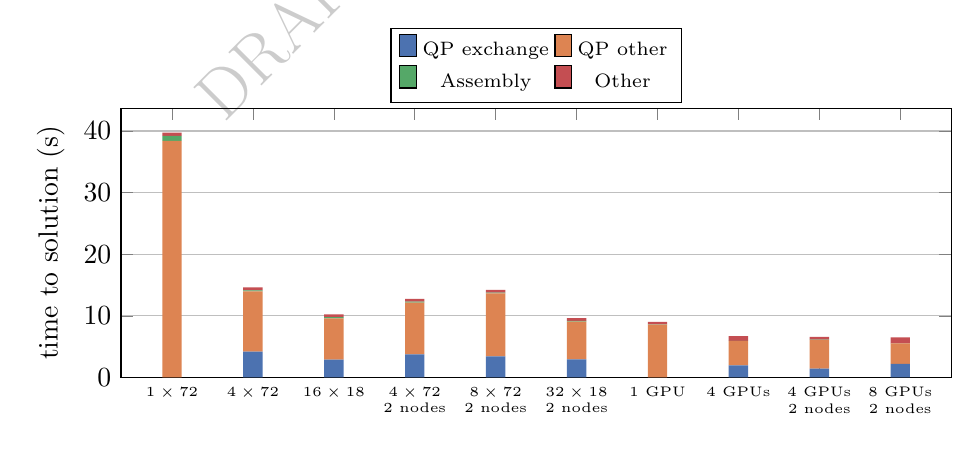
\begin{tikzpicture}
\begin{axis}[ybar stacked, bar width=7pt, width=\columnwidth, height=5.0cm,
  symbolic x coords={c0,c1,c2,c3,c4,c5,c6,c7,c8,c9}, xtick=data,
  xticklabels={{$1\times72$},{$4\times72$},{$16\times18$},{$4\times72$\\2 nodes},{$8\times72$\\2 nodes},{$32\times18$\\2 nodes},{1 GPU},{4 GPUs},{4 GPUs\\2 nodes},{8 GPUs\\2 nodes}}, xticklabel style={font=\tiny, align=center},
  ymin=0, ylabel={time to solution (\si{\second})}, ymajorgrids,
  legend style={font=\scriptsize, at={(0.5,1.02)}, anchor=south, legend columns=2},
  enlarge x limits=0.07]
\addplot[fill=LdpA, draw=none] coordinates {(c0,0.000) (c1,4.181) (c2,2.879) (c3,3.738) (c4,3.398) (c5,2.932) (c6,0.000) (c7,1.947) (c8,1.430) (c9,2.210)};
\addlegendentry{QP exchange}
\addplot[fill=LdpB, draw=none] coordinates {(c0,38.418) (c1,9.785) (c2,6.693) (c3,8.408) (c4,10.256) (c5,6.125) (c6,8.584) (c7,3.987) (c8,4.677) (c9,3.301)};
\addlegendentry{QP other}
\addplot[fill=LdpC, draw=none] coordinates {(c0,0.799) (c1,0.176) (c2,0.210) (c3,0.173) (c4,0.109) (c5,0.122) (c6,0.009) (c7,0.004) (c8,0.004) (c9,0.003)};
\addlegendentry{Assembly}
\addplot[fill=LdpD, draw=none] coordinates {(c0,0.513) (c1,0.464) (c2,0.451) (c3,0.433) (c4,0.436) (c5,0.452) (c6,0.416) (c7,0.747) (c8,0.473) (c9,0.967)};
\addlegendentry{Other}
\end{axis}
\end{tikzpicture}

\caption{Time to solution of FF200 refined (\dofsFFf{} dofs) by phase.}
\label{fig:breakdown}
\end{figure}

Table~\ref{tab:performance} and Figure~\ref{fig:per-iteration} give the cost per QP iteration and
the time to solution. The QP accounts for at least \qpShareFFf\% of the solve time on FF200 refined
in every configuration (Figure~\ref{fig:breakdown}), so the cost per QP iteration determines the
time to solution.

\paragraph{GPUs.} One GPU is the fastest configuration on \oneGpuBestCases{}; \bestElsewhere{}. Per case, the fastest Grace configuration takes
\gpuOverGraceMin{} to \gpuOverGraceMax{} times as long as the fastest GPU configuration.

\paragraph{Grace.} An empty OpenMP parallel region costs \regionCostWide\,\si{\micro\second} with
\machineCores{} threads per rank and \regionCostNarrow\,\si{\micro\second} with 18, as much as a pass
over a rank's unknowns. MPRGP's conjugate-gradient steps therefore share one region, and a QP
iteration of FF200 on $1\times72$ opens \regionsPerIteration{}. Their sums are not OpenMP reduction
clauses: GCC combines a clause of several variables under a global lock of its runtime, on which
the threads of a rank serialise. In a stand-in for the step on FF200's unknowns, with a
tridiagonal matrix in place of the tangent, a region per pass with such clauses costs
\standinRegionsOne{} and \standinRegionsFour\,\si{\micro\second} per step on $1\times72$ and
$4\times72$, one shared region \standinTeamOne{} and \standinTeamFour\,\si{\micro\second}. On one
node $4\times72$ costs \hostThreadsMin{} to \hostThreadsMax{} times as much per iteration as
$16\times18$, and more than $1\times72$ only on \fourSlowerThanOneCases{}, the case with the least
work per rank, where the stand-in's synchronisation accounts for \standinGap{} of the
\hostGapOneFour\,\si{\micro\second} difference.

\paragraph{Latency.} The cheapest iteration of each case costs \itBestMin{} to
\itBestMax\,\si{\micro\second}, while the work per iteration grows \dofsRatio-fold from the smallest
to the largest case: the QP iteration is latency bound. Its fixed cost is the two global reductions, the
ghost exchange, on Grace the three barriers and, on the GPU, the kernel launches and the transfer of each reduction's result to
the host. Adding ranks shrinks the work per rank but not these costs, which bounds the strong
scaling of every case.

\paragraph{Reference.} Utopia solved the four cases in \utopiaTimeFPc, \utopiaTimeFFc,
\utopiaTimeFPf{} and \utopiaTimeFFf\,\si{\second} on \utopiaRanks{} MPI ranks of an unrecorded
machine, with \utopiaNewtonFPc, \utopiaNewtonFFc, \utopiaNewtonFPf{} and \utopiaNewtonFFf{} Newton
steps. Without the machine and at different accuracies the times are no basis for a speed-up.

\paragraph{Load steps.} The overlap can instead be released over $n$ quasi-static pseudo-steps:
the bound admits a share of the starting penetration that falls linearly to zero, and each
pseudo-step is solved to convergence. Table~\ref{tab:release} compares $n=1$, 2 and 4 on
$4\times72$, with utopia's damped step and with full Newton steps under an Armijo line search; a
pseudo-step whose line search fails is retried with half its length. With the damped step a
pseudo-step takes \releasePerStepMin{} to \releasePerStepMax{} times as many Newton steps as the
single step, so two pseudo-steps take \releaseTwoMin{} to \releaseTwoMax{} and four
\releaseFourMin{} to \releaseFourMax{} times as long. In one step the Armijo rule solves
\armijoFasterCases{} \armijoGainMin{} to \armijoGainMax\% faster than the damped step, but on
\armijoCutbackCase{} its line search fails in every repeat and the retry makes the solve
\armijoCutbackSlower{} times as long. \armijoCutbackRuns{} of the \armijoRuns{} Armijo runs were
retried, none of the damped ones. The cases therefore remove the overlap in one damped step.

\paragraph{Single-precision tangent.} The tangent's values can be stored in single precision. Each
entry of an element matrix is computed in double and rounded once as it is added, so the matrix is
assembled in this format directly, without a copy in double; the operator application reads the
values into double and accumulates in double, and the vectors and the QP stay in double. This
halves the bytes of matrix values each operator application reads. Table~\ref{tab:precision}
compares the two precisions on one node in \precisionRuns{} runs that alternate between them per
repeat, with the build of Table~\ref{tab:performance}. Single precision lowers the cost per QP
iteration by \singleGpuOneMin{} to \singleGpuOneMax\% on one GPU, and on FF200 refined by
\singleRefinedGrace\% on $16\times18$ and \singleRefinedFour\% on four GPUs; there one GPU solves in
\solveSingleFFfGpuOne{} instead of \solveDoubleFFfGpuOne\,\si{\second}. With several ranks on the
smaller cases the change lies between \singleSmallMin{} and \singleSmallMax\%. The Newton step
counts are unchanged, and the median QP iteration count changes by at most \singleQpChange\%; in
\singleQpOutside{} of \singleQpConfigs{} configurations that is more than the spread between the
three double repeats, by at most \singleQpExcess{} percentage points. In the same configuration
the final displacement in single precision differs from the first double run by at most a
relative \agreeSingle{} on \convergedCases{}, while the double repeats differ from each other by
up to \agreeDouble{}; on \unconvergedCases{} the two figures are \agreeSingleUnconverged{} and
\agreeDoubleUnconverged{}. Double precision remains the default and is used everywhere else in
this paper.

\paragraph{Communication within a node.} As an option, the GPUs of one node exchange ghost values
by NCCL~\cite{nccl}, queued on the GPU's stream, and, where one node holds every rank, MPRGP's two
reductions complete on the GPU as well, so that an iteration returns to the host once, as on one
GPU. Between nodes GPU-aware MPI remains for both: there NCCL's messages took longer than MPI's
and, unless libfabric sends every message by rendezvous, delivered wrong values; with rendezvous,
its reductions over two nodes saved no time. Table~\ref{tab:nccl} compares the option with MPI in
\ncclRuns{} runs alternating per repeat; the Newton step counts are the same. On one node NCCL
lowers the cost per QP iteration by \ncclOneGainMin{} to \ncclOneGainMax\%, on two nodes, eight
GPUs, by \ncclEightGainMin{} to \ncclEightGainMax\%. Its set-up takes \ncclInitMin{} to
\ncclInitMax\,\si{\second} once per process, most of it in calls to the GPU driver, on a thread of
its own beside the rest of the set-up; the run waits for it, or is slowed by it, for
\ncclCostMin{} to \ncclCostMax\,\si{\second}, and the time to solution grows by \ncclExtraMin{}
to \ncclExtraMax\,\si{\second} on every case. The option repays its set-up after
\ncclBreakEvenMin{} to \ncclBreakEvenMax{} QP iterations a process. It is off by default.

\begin{table*}
\caption{Cost per QP iteration (\si{\micro\second}) and time to solution (\si{\second}), median of
\benchRepeats{} runs. Grace configurations are ranks $\times$ threads.}
\label{tab:performance}
\small
%% Generated by wip/ldp_containment/python/ldp_figures.py -- do not edit.
%% Regenerate with: make figures

\begin{tabular}{@{}llrrrrrrrr@{}}
\toprule
 & & \multicolumn{2}{c}{FF200} & \multicolumn{2}{c}{FP70 coarse} & \multicolumn{2}{c}{FP70} & \multicolumn{2}{c}{FF200 refined} \\
\cmidrule(lr){3-4}\cmidrule(lr){5-6}\cmidrule(lr){7-8}\cmidrule(lr){9-10}
Nodes & Configuration & \si{\micro\second} & \si{\second} & \si{\micro\second} & \si{\second} & \si{\micro\second} & \si{\second} & \si{\micro\second} & \si{\second} \\
\midrule
1 & $1\times72$ & \num{218} & \num{3.23} & \num{257} & \num{4.52} & \num{582} & \num{3.18} & \num{1317} & \num{39.7} \\
1 & $4\times72$ & \num{299} & \num{4.14} & \num{299} & \num{5.02} & \num{356} & \num{1.92} & \num{488} & \num{14.6} \\
1 & $16\times18$ & \num{159} & \num{2.33} & \num{175} & \num{3.13} & \num{226} & \num{1.51} & \num{341} & \num{10.2} \\
\addlinespace
2 & $4\times72$ & \num{247} & \num{3.42} & \num{304} & \num{5.01} & \num{297} & \num{1.80} & \num{423} & \num{12.8} \\
2 & $8\times72$ & \num{369} & \num{4.95} & \num{343} & \num{5.68} & \num{397} & \num{2.20} & \num{493} & \num{14.2} \\
2 & $32\times18$ & \num{228} & \num{3.10} & \num{223} & \num{3.61} & \num{255} & \num{1.61} & \num{330} & \num{9.63} \\
\addlinespace
1 & 1 GPU & \num{102} & \num{1.54} & \num{118} & \num{2.07} & \num{202} & \num{1.23} & \num{304} & \num{9.01} \\
1 & 4 GPUs & \num{139} & \num{2.32} & \num{142} & \num{2.98} & \num{183} & \num{1.71} & \num{207} & \num{6.69} \\
\addlinespace
2 & 4 GPUs & \num{141} & \num{2.12} & \num{142} & \num{2.69} & \num{176} & \num{1.21} & \num{212} & \num{6.58} \\
2 & 8 GPUs & \num{172} & \num{3.00} & \num{186} & \num{3.76} & \num{190} & \num{1.80} & \num{197} & \num{6.48} \\
\bottomrule
\end{tabular}

\end{table*}

\begin{table*}
\caption{The tangent in double and in single precision on one node: cost per QP iteration and
time to solution, median of \benchRepeats{} runs each.}
\label{tab:precision}
\small
\setlength{\tabcolsep}{3.5pt}
%% Generated by wip/ldp_containment/python/ldp_figures.py -- do not edit.
%% Regenerate with: make figures

\begin{tabular}{@{}llrrrrr@{}}
\toprule
 & & \multicolumn{3}{c}{\si{\micro\second} per QP iteration} & \multicolumn{2}{c}{Solve (\si{\second})} \\
\cmidrule(lr){3-5}\cmidrule(l){6-7}
Case & Configuration & double & single & change & double & single \\
\midrule
FF200 & $16\times18$ & \num{136} & \num{135} & \num{-0.0}\% & \num{2.12} & \num{2.08} \\
 & 1 GPU & \num{86} & \num{67} & \num{-21.6}\% & \num{1.38} & \num{1.15} \\
 & 4 GPUs & \num{134} & \num{133} & \num{-1.0}\% & \num{2.33} & \num{2.29} \\
\addlinespace
FP70 coarse & $16\times18$ & \num{160} & \num{156} & \num{-2.2}\% & \num{2.86} & \num{2.81} \\
 & 1 GPU & \num{98} & \num{81} & \num{-17.0}\% & \num{1.75} & \num{1.57} \\
 & 4 GPUs & \num{135} & \num{135} & \num{-0.0}\% & \num{2.95} & \num{2.97} \\
\addlinespace
FP70 & $16\times18$ & \num{208} & \num{201} & \num{-3.2}\% & \num{1.25} & \num{1.31} \\
 & 1 GPU & \num{176} & \num{145} & \num{-17.7}\% & \num{1.09} & \num{0.992} \\
 & 4 GPUs & \num{174} & \num{169} & \num{-2.9}\% & \num{1.56} & \num{1.54} \\
\addlinespace
FF200 refined & $16\times18$ & \num{314} & \num{267} & \num{-15.0}\% & \num{9.28} & \num{8.30} \\
 & 1 GPU & \num{279} & \num{225} & \num{-19.4}\% & \num{8.61} & \num{6.62} \\
 & 4 GPUs & \num{199} & \num{178} & \num{-10.6}\% & \num{6.36} & \num{6.10} \\
\bottomrule
\end{tabular}

\end{table*}

\begin{table*}
\caption{Communication within a node by MPI and by NCCL: cost per QP iteration, what NCCL's set-up
costs a run (the longer set-up and the wait at the first communication) and the QP iterations
that repay it, and time to solution (set-up and solve), median of \benchRepeats{} runs each.}
\label{tab:nccl}
\small
%% Generated by wip/ldp_containment/python/ldp_figures.py -- do not edit.
%% Regenerate with: make figures

\begin{tabular}{@{}llrrrrr@{}}
\toprule
 & & \multicolumn{3}{c}{\si{\micro\second} per QP iteration} & \multicolumn{2}{c}{To solution (\si{\second})} \\
\cmidrule(lr){3-5}\cmidrule(l){6-7}
Case & Configuration & MPI & NCCL & change & MPI & NCCL \\
\midrule
FF200 & 4 GPUs & \num{134} & \num{97} & \num{-27.3}\% & \num{6.69} & \num{9.49} \\
 & 4 GPUs, 2 nodes & \num{131} & \num{130} & \num{-1.2}\% & \num{2.66} & \num{3.91} \\
 & 8 GPUs, 2 nodes & \num{160} & \num{135} & \num{-15.5}\% & \num{3.43} & \num{6.90} \\
\addlinespace
FP70 coarse & 4 GPUs & \num{136} & \num{97} & \num{-28.3}\% & \num{7.01} & \num{10.0} \\
 & 4 GPUs, 2 nodes & \num{132} & \num{134} & \num{1.7}\% & \num{2.82} & \num{4.34} \\
 & 8 GPUs, 2 nodes & \num{172} & \num{138} & \num{-20.1}\% & \num{3.80} & \num{7.37} \\
\addlinespace
FP70 & 4 GPUs & \num{176} & \num{147} & \num{-16.3}\% & \num{5.89} & \num{9.30} \\
 & 4 GPUs, 2 nodes & \num{163} & \num{171} & \num{4.6}\% & \num{1.76} & \num{3.35} \\
 & 8 GPUs, 2 nodes & \num{175} & \num{149} & \num{-15.1}\% & \num{2.07} & \num{6.12} \\
\addlinespace
FF200 refined & 4 GPUs & \num{201} & \num{185} & \num{-7.9}\% & \num{11.5} & \num{14.0} \\
 & 4 GPUs, 2 nodes & \num{194} & \num{210} & \num{8.0}\% & \num{7.51} & \num{9.39} \\
 & 8 GPUs, 2 nodes & \num{182} & \num{170} & \num{-6.5}\% & \num{7.13} & \num{10.5} \\
\bottomrule
\end{tabular}

\end{table*}

\begin{table*}
\caption{The overlap released over 1, 2 and 4 pseudo-steps, each solved to convergence, on
$4\times72$: Newton steps (those of failed attempts included) and solve time, median of
\releaseRepeats{} runs each, alternating per repeat.}
\label{tab:release}
\small
%% Generated by wip/ldp_containment/python/ldp_figures.py -- do not edit.
%% Regenerate with: make figures

\begin{tabular}{@{}llrrrrrr@{}}
\toprule
 & & \multicolumn{2}{c}{1 step} & \multicolumn{2}{c}{2 steps} & \multicolumn{2}{c}{4 steps} \\
\cmidrule(lr){3-4}\cmidrule(lr){5-6}\cmidrule(lr){7-8}
Case & Line search & Newton & \si{\second} & Newton & \si{\second} & Newton & \si{\second} \\
\midrule
FF200 & damped & \num{20} & \num{1.74} & \num{38} & \num{3.50} & \num{85} & \num{7.46} \\
 & Armijo & \num{17} & \num{1.40} & \num{35} & \num{2.84} & \num{63} & \num{6.02} \\
\addlinespace
FP70 coarse & damped & \num{13} & \num{2.38} & \num{28} & \num{4.61} & \num{60} & \num{9.04} \\
 & Armijo & \num{25} & \num{6.51} & \num{22} & \num{3.22} & \num{45} & \num{6.31} \\
\addlinespace
FP70 & damped & \num{13} & \num{3.93} & \num{26} & \num{8.44} & \num{55} & \num{15.9} \\
 & Armijo & \num{9} & \num{3.01} & \num{31} & \num{6.24} & \num{55} & \num{12.0} \\
\addlinespace
FF200 refined & damped & \num{16} & \num{9.84} & \num{33} & \num{18.4} & \num{59} & \num{37.9} \\
 & Armijo & \num{12} & \num{6.63} & \num{23} & \num{12.5} & \num{48} & \num{26.2} \\
\bottomrule
\end{tabular}

\end{table*}

\begin{figure*}
\centering
%% Generated by wip/ldp_containment/python/ldp_figures.py -- do not edit.
%% Regenerate with: make figures

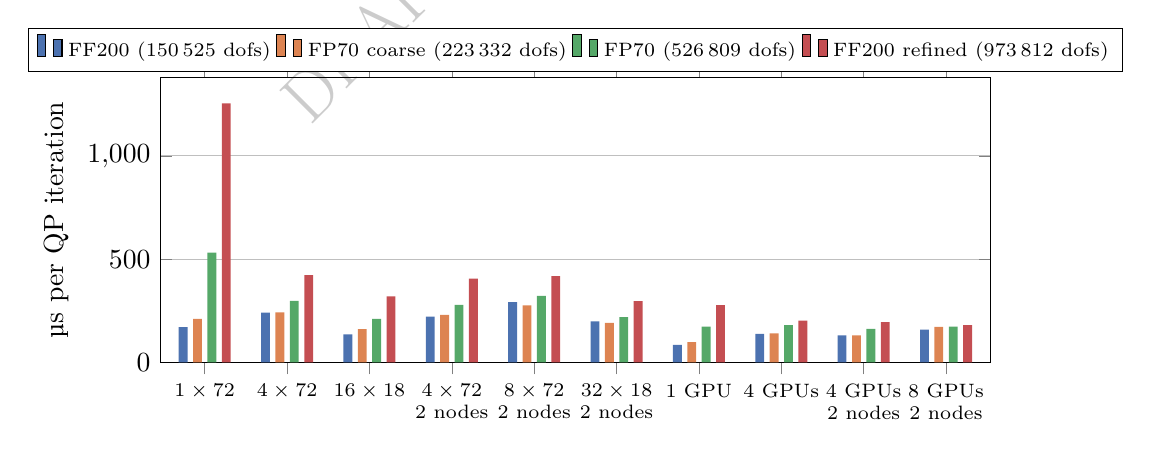
\begin{tikzpicture}
\begin{axis}[ybar, bar width=3.2pt, width=\textwidth, height=5.2cm,
  symbolic x coords={c0,c1,c2,c3,c4,c5,c6,c7,c8,c9}, xtick=data,
  xticklabels={{$1\times72$},{$4\times72$},{$16\times18$},{$4\times72$\\2 nodes},{$8\times72$\\2 nodes},{$32\times18$\\2 nodes},{1 GPU},{4 GPUs},{4 GPUs\\2 nodes},{8 GPUs\\2 nodes}}, xticklabel style={font=\scriptsize, align=center},
  ymin=0, ylabel={\si{\micro\second} per QP iteration}, ymajorgrids,
  legend style={font=\scriptsize, at={(0.5,1.02)}, anchor=south, legend columns=4},
  enlarge x limits=0.06]
\addplot[fill=LdpA, draw=none] coordinates {(c0,171.0) (c1,241.5) (c2,136.7) (c3,221.6) (c4,292.3) (c5,199.4) (c6,85.5) (c7,138.5) (c8,131.0) (c9,159.1)};
\addlegendentry{FF200 (\num{150525} dofs)}
\addplot[fill=LdpB, draw=none] coordinates {(c0,211.5) (c1,243.0) (c2,162.0) (c3,230.3) (c4,276.3) (c5,192.3) (c6,98.8) (c7,141.0) (c8,131.7) (c9,172.4)};
\addlegendentry{FP70 coarse (\num{223332} dofs)}
\addplot[fill=LdpC, draw=none] coordinates {(c0,531.2) (c1,298.7) (c2,210.9) (c3,278.4) (c4,322.4) (c5,219.6) (c6,173.2) (c7,181.1) (c8,163.0) (c9,173.8)};
\addlegendentry{FP70 (\num{526809} dofs)}
\addplot[fill=LdpD, draw=none] coordinates {(c0,1253.5) (c1,423.0) (c2,320.3) (c3,405.4) (c4,418.2) (c5,296.7) (c6,277.5) (c7,203.1) (c8,195.8) (c9,181.3)};
\addlegendentry{FF200 refined (\num{973812} dofs)}
\end{axis}
\end{tikzpicture}

\caption{Cost per QP iteration of every configuration.}
\label{fig:per-iteration}
\end{figure*}

\section{Limitations}

In the single-process runs \qpCappedClause{}. The Newton budget
of \unconvergedCases{} ends before the KKT tolerance is reached. The comparison with utopia samples
the distance field trilinearly for both states, so penetrations below the grid's interpolation
error are not resolved. All measurements are on one system; utopia was not rerun on it.

\bibliographystyle{ACM-Reference-Format}
\bibliography{refs}

\end{document}
